%% This is an example first chapter.  You should put chapter/appendix that you
%% write into a separate file, and add a line \include{yourfilename} to
%% main.tex, where `yourfilename.tex' is the name of the chapter/appendix file.
%% You can process specific files by typing their names in at the 
%% \files=
%% prompt when you run the file main.tex through LaTeX.
\chapter{Project Management}

\section{Planning}

The project started on September 2013 with full-time dedication on it was planned to be finished by the 2th of December 2013. The first steps were to study its feasibility in terms of technology, to outline the vision and specify the requirements with CREAF. Next steps included the design and implementation of the identified major components of the solution. It would end with the infrastructure setup, testing and the writing of the current document.

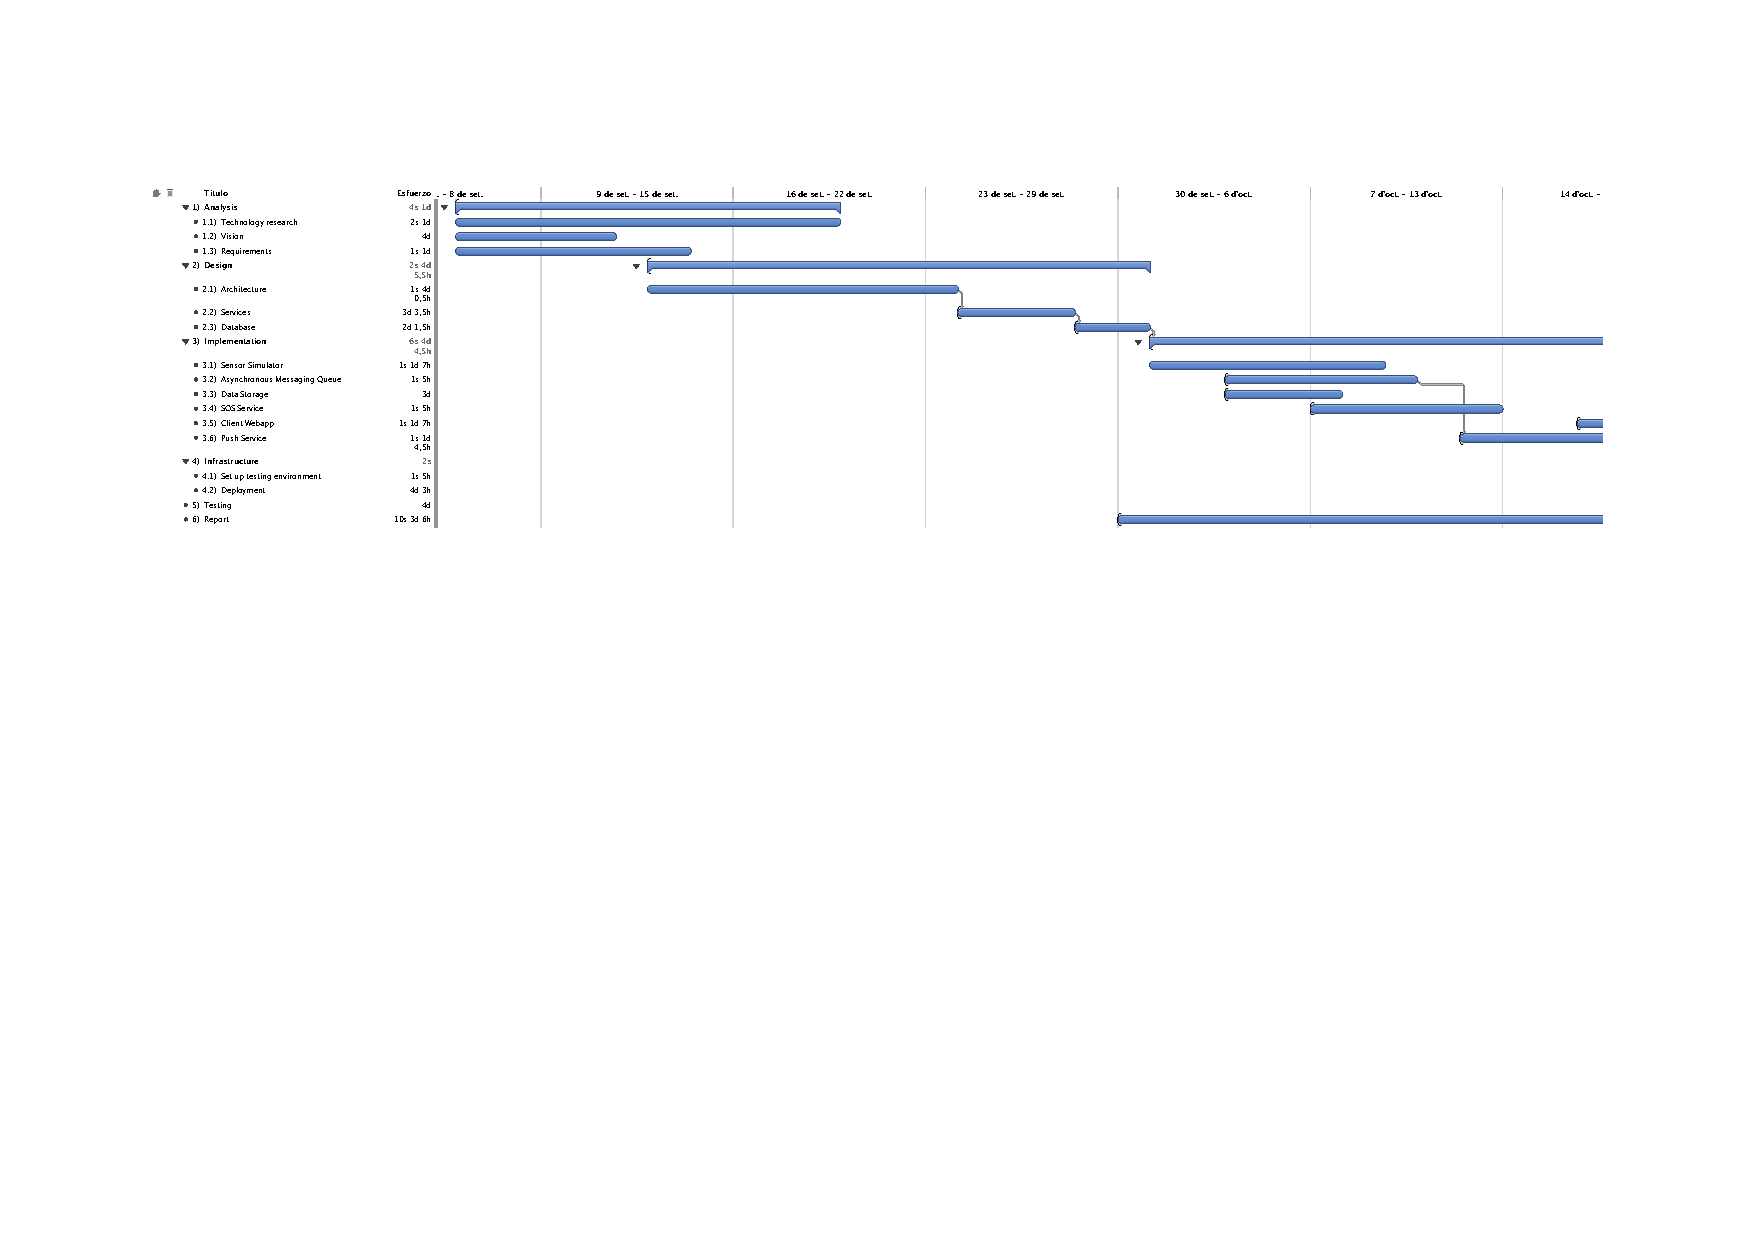
\includepdf[landscape=true, pages={1-2}]{initial_planning}

\section{Cost}

In order to forecast the cost must be considered the resources involved in the project and their cost. These are an analyst, who will be in charge of the Analysis and Design, a Developer, who will implement the design and a System administrator, who will set up the infrastructure.

Considering these roles and the initial planning the overall cost is $15150\euro{}$

\begin{table}[H]
    \centering
    \begin{tabular}{| l | l | l | l |}
    \hline
    \textbf{Resource}  & \textbf{Cost/Hour}  & \textbf{Hours}  & \textbf{Cost} \\ \hline
    Analyst            & 40\euro{}/h         & 200             & 8000\euro{}   \\ \hline
    Developer          & 25\euro{}/h         & 250             & 6250\euro{}   \\ \hline
    SysAdmin           & 20\euro{}/h         & 45              & 900\euro{}    \\ \hline
    \textbf{Overall}   &                     &                 & \textbf{15150\euro{}} \\ \hline
    \end{tabular}
    \caption{Budget}
    \label{tab:budget}
\end{table}

\section{Execution}

\section{PaaS and IaaS cost comparison}